\PassOptionsToPackage{table}{xcolor}
\ifbeamerarticle
  \documentclass[12pt]{article}
  \usepackage{beamerarticle}
\else
  \documentclass[12pt]{beamer}
\fi
% Packages
\usepackage{mflogo}
\usepackage{tikz}
\usetikzlibrary{fadings,patterns}
\usepackage{pgfplots}
\pgfplotsset{compat=1.8}
\usepgfplotslibrary{statistics}
\usepackage{polyglossia}
\setmainlanguage{english}
\usepackage{tabularx}
\usepackage{booktabs}
\usepackage{placeins}
%% Bibliography
\usepackage[
  backend=biber,
  style=numeric,
  citestyle=numeric-comp,
  sorting=none
]{biblatex}
\addbibresource{../database.bib}
\ifbeamerarticle
  \let\mycite\cite
\else
  \let\mycite\footfullcite
\fi
%% Fonts
\usepackage{fontspec}
\ifbeamerarticle
  \usepackage{mathpazo}
\else
  \usepackage{cmbright}
\fi
\setmainfont[Ligatures=TeX]{Comenia Serif}
\setsansfont[Ligatures=TeX]{Comenia Sans}
\setmonofont[Scale=MatchLowercase,Ligatures=TeX]{Inconsolata}
\ifbeamerarticle
  \def\pkg#1{{\sf#1}}
\else
  \let\pkg\emph
\fi
%% Hyperref
\makeatletter
  \@ifpackageloaded{hyperref}{}{\usepackage{hyperref}}
\makeatother
\hypersetup{\ifbeamerarticle color\else hide\fi links,
  linkcolor=black}
% Theming & colors
\usetheme{Antibes}
\usecolortheme{crane}
\usefonttheme{professionalfonts}
\definecolor{green}{RGB}{0,130,0}
\definecolor{yellow}{RGB}{242,212,92}
\definecolor{orange}{RGB}{255,100,0}
% Tabular redefinition
\def\redefinetables{%
  \definecolor{tableOdd}{HTML}{FFF9E5}
  \definecolor{tableEven}{HTML}{FFECB3}
  \definecolor{tableEmph}{HTML}{FFD451}
  \let\oldtabular\tabular
  \let\endoldtabular\endtabular
  \renewenvironment{tabular}%
    {\rowcolors{1}{tableOdd}%
                  {tableEven}%
     \oldtabular}%
    {\endoldtabular}
  \let\oldtabularx\tabularx
  \let\endoldtabularx\endtabularx
  \renewenvironment{tabularx}%
    {\rowcolors{1}{tableOdd}%
                  {tableEven}%
     \oldtabularx}%
     {\endoldtabularx}}
\setlength{\aboverulesep}{0pt}
\setlength{\belowrulesep}{0pt}
\setlength{\extrarowheight}{.75ex}
\def\cellemph{\cellcolor{tableEmph}}
\def\rowemph{\rowcolor{tableEmph}}

% Miscellanea
\frenchspacing
\ifbeamerarticle\else
  \beamertemplatenavigationsymbolsempty
  \setbeamertemplate{caption}[numbered]
\fi
% Section front page support
\AtBeginSection{\frame{\sectionpage}}
\AtBeginSubsection{\frame{\subsectionpage}}
% Nested itemize fix
% http://tex.stackexchange.com/a/74069/70941
\ifbeamerarticle\else
  \usepackage{etoolbox}
  \setbeamercovered{transparent}
  \makeatletter
  \newcommand*\fix@beamer@close{%
    \ifnum\beamer@trivlistdepth>0%
      \beamer@closeitem%
    \fi}
  \newcommand*\fix@beamer@open{%
    \ifnum\beamer@trivlistdepth>0%
      \gdef\beamer@closeitem{}%
    \fi}
  \BeforeBeginEnvironment{enumerate}{\fix@beamer@close}
  \AfterEndEnvironment{enumerate}{\fix@beamer@open}
  \BeforeBeginEnvironment{itemize}{\fix@beamer@close}
  \AfterEndEnvironment{itemize}{\fix@beamer@open}
  \BeforeBeginEnvironment{description}{\fix@beamer@close}
  \AfterEndEnvironment{description}{\fix@beamer@open}
  \makeatother
\fi
% Metadata
\title{The Form of Theses\\ Written in \LaTeX}
\subtitle{Thesis Presentation}
\date{May 28, 2015}
\author{Vít Novotný}
\institute[FI MU]{Faculty of Informatics,\\Masaryk University in
  Brno}
\begin{document}
\frame{\maketitle}
\frame{\tableofcontents}
\redefinetables\clearpage
\section{\TeX\ Usage at MU}
\newlength\yearposx
\begin{frame}[label=history]
  \frametitle{History}
    \begin{itemize}[<+->]
    \item \textcolor{violet}{1994} -- The \textcolor{violet}{ 
      logo} of FI MU \mycite{zlatuska95}
    \item \textcolor{red}{1998--2008} -- The
      \textcolor{red}{\pkg{fithesis1}} class
    \item \textcolor{green}{2001--2004} -- The
      \textcolor{green}{\pkg{xslt2}} module
    \item \textcolor{blue}{2008--2015} -- The
      \textcolor{blue}{\pkg{fithesis2}} class
    \item \textcolor{orange}{2013} -- The
      \textcolor{orange}{\pkg{comenia}} package
  \end{itemize}\medskip
  \begin{tikzpicture}[remember picture,overlay]
    \node [anchor=east] at (\ifbeamerarticle13\else11\fi cm,
    \ifbeamerarticle4.8\else2.25\fi cm) {
      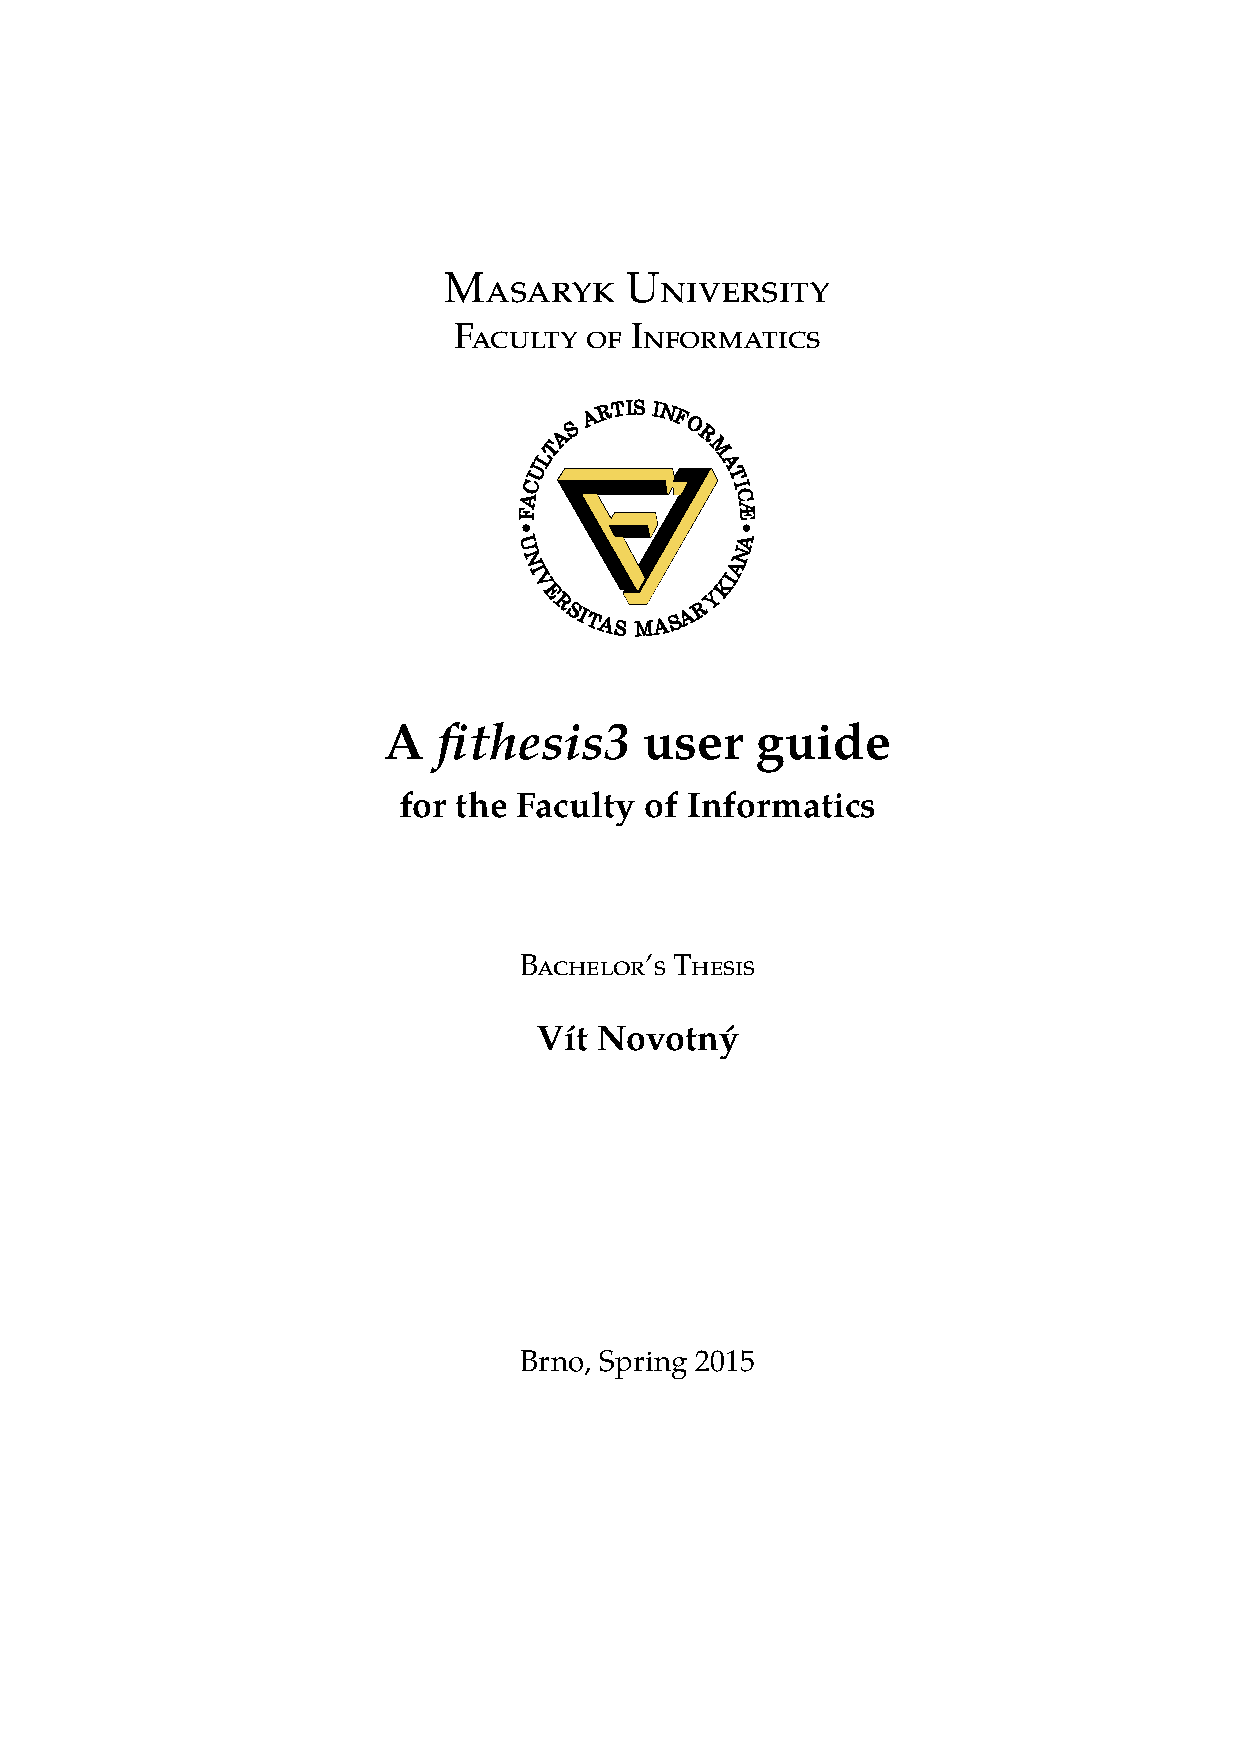
\includegraphics[width=\ifbeamerarticle4\else3.2\fi cm]
      {../fithesis3/fithesis3/logo/mu/color/fi}};
  \end{tikzpicture}
  \begin{tikzpicture}[scale=\ifbeamerarticle0.585\else0.46\fi]
    \foreach \x in {1994,1998,2001,2004,2008,2013,2015}{
      \pgfmathsetlength\yearposx{(\x-1994)*1cm};
      \coordinate (y\x) at (\yearposx,0);
      \coordinate (y\x t) at (\yearposx,0.75mm);
      \draw (\yearposx,+3pt) -- (\yearposx,-3pt);}
    \draw [->] (y1994) -- (y2015);
    \uncover<1-> {\node at (y1994) [above=3pt]
      {\textcolor{violet}{1994}};}
    \only<1-> {\fill[violet] (y1994) circle (5pt);}
    \uncover<2-> {
      \node at (y1998) [below=3pt] {\textcolor{red}{1998}};}
    \uncover<2-4> {\node at (y2008) [above=3pt]
      {\textcolor{red}{2008}};}
    \only<2-> {
      \draw[red,very thick] (y1998) -- (y2008);
      \fill[red] (y1998) circle (5pt);
      \fill[red] (y2008) circle (5pt);}
    \uncover<3-> {
      \node at (y2001) [above=3pt] {\textcolor{green}{2001}};
      \node at (y2004) [below=3pt] {\textcolor{green}{2004}};}
    \only<3-> {
      \draw[green,very thick] (y2001t) -- (y2004t);
      \fill[green] (y2001t) circle (5pt);
      \fill[green] (y2004t) circle (5pt);}
    \uncover<4-> {
      \node at (y2015) [below=3pt] {\textcolor{blue}{2015}};}
    \only<4-> {
      \node at (y2008) [above=3pt] {
        \textcolor{blue!0!red}2%
        \textcolor{blue!33!red}0%
        \textcolor{blue!66!red}0%
        \textcolor{blue!100!red}8};
      \draw[blue,very thick] (y2008) -- (y2015);
      \fill[blue] (y2008) circle (5pt);
      \fill[blue] (y2015) circle (5pt);}
    \uncover<5-> {\node at (y2013) [above=3pt]
      {\textcolor{orange}{2013}};}
    \only<5-> {\fill[orange] (y2013t) circle (5pt);}
  \end{tikzpicture}
\end{frame}
\subsection{User Survey}
\begin{frame}[c]
  \begin{table}[!b]
    \begin{tabularx}{\textwidth}{Xcr}
      \textbf{On which faculty of
      MU do you study?} & \textbf{\#}
      \\ \toprule Faculty of Informatics          & $82$
      \\ Faculty of Science                       &  $3$
      \\ Faculty of Education                     &  $2$
      \\ Faculty of Social Studies                &  $2$
      \\ Faculty of Law                           &  $1$
      \\ Faculty of Medicine                      &  $1$
      \\ Faculty of Arts                          &  $1$
      \\ Faculty of Economics and Administration  &  $1$
      \\ Faculty of Sports Studies                &  $0$
      \\
    \end{tabularx}
    \caption{The distribution of the questionnaire
      respondents across the faculties of MU}
  \end{table}
\end{frame}
\begin{frame}[c]
  \begin{table}[!b]
    \begin{tabularx}{\textwidth}{Xcr}
      \textbf{Which academic degree are you pursuing?} &
      \textbf{\#} \\
      \toprule
      Bachelor's degree  & $70$ \\
      Master's degree    & $17$ \\
      Doctorate          & $2$  \\
      \bottomrule
      \textbf{Total}     & $\mathbf{89}$
    \end{tabularx}
    \caption{The highest academic degrees currently pursued by the
      respondents of the questionnaire}
  \end{table}
\end{frame}
\begin{frame}
  \begin{table}[!b]
    \begin{tabularx}{\textwidth}{Xcr}
      \textbf{Which application do you use / are you planning to
      use to write your thesis?} & \textbf{\#} \\
      \toprule
      \TeX\ / \LaTeX          & $65$          \\
      Microsoft Office        & $16$          \\
      Apache OpenOffice, LibreOffice or another free office
      software suite          & $4$           \\
      Other                   & $4$           \\
      Google Documents        & $0$           \\
      \bottomrule
      \textbf{Total}          & $\mathbf{89}$ 
    \end{tabularx}
    \caption{The software the respondents of the questionnaire
      were using or planning to use to write their theses}
  \end{table}
\end{frame}
\begin{frame}
  \begin{table}[!b]
    \begin{tabularx}{\textwidth}{Xcr}
      \textbf{Are you planning to use the \pkg{fithesis1}
        class?} & \textbf{\#} \\
      \toprule    Yes                       & $47$
      \\ Maybe, I did not know it existed   & $10$
      \\ No, I'm going to use another class & $5$
      \\ Other                              & $2$
      \\ No, I'm going to use plain \TeX{}  & $1$
      \\ \bottomrule
      \textbf{Total}  & $\mathbf{65}$ 
    \end{tabularx}
      \caption{The attitude towards the usage of the \pkg{fithesis1}
      class amongst those respondents who claimed to be using or
      planning to use \TeX{} to typeset their theses}
  \end{table}
\end{frame}\FloatBarrier
\begin{frame}
  \frametitle{Conclusion}
  The majority of respondents:
  \begin{itemize}
    \item Were FI bachelor's degree students.
    \item Preferred \pkg{fithesis1} over the alternatives.
  \end{itemize}
\end{frame}
\subsection{Analysis of Existing Theses}
\begin{frame}
  \begin{table}[!b]
    \scalebox{\ifbeamerarticle1\else0.9\fi}{\begin{tabularx}%
      {\ifbeamerarticle1\else1.11\fi\textwidth}{Xrr}
      \textbf{Faculty} & \textbf{\#} & \textbf{\%} \\
      \toprule
      Faculty of Arts                         & $10\,000$ & $21.98$ \\% 1421
      Faculty of Education                    & $8\,219$  & $18.07$ \\% 1441
      Faculty of Social Studies               & $5\,599$  & $12.31$ \\% 1423
      Faculty of Science                      & $5\,275$  & $11.60$ \\% 1431
      Faculty of Law                          & $4\,824$  & $10.60$ \\% 1422
      Faculty of Economics and Administration & $4\,591$  & $10.09$ \\% 1456
      Faculty of Informatics                  & $2\,904$  &  $6.38$ \\% 1433
      Faculty of Medicine                     & $2\,014$  &  $4.43$ \\% 1411
      Faculty of Sports Studies               & $2\,062$  &  $4.53$ \\% 1451
      \bottomrule
      \textbf{Total}     & $\mathbf{45\,488}$ & $\mathbf{100.00}$
    \end{tabularx}}
    \caption{The distribution of theses defended between 2010--2015
      across the faculties of MU}
  \end{table}
\end{frame}
\begin{frame}
  \begin{table}[!b]
    \begin{tabularx}{\textwidth}{Xrr}
      \textbf{Degree} & \textbf{\#} & \textbf{\%} \\
      \toprule
      Bachelor's & $22\,288$ & $49.00$ \\
      Master's   & $20\,761$ & $45.64$ \\
      Doctoral   &  $2\,231$ &  $4.90$ \\
      Lifelong   &     $208$ &  $0.46$ \\
      \bottomrule
      \textbf{Total} & $\mathbf{45\,488}$ & $\mathbf{100.00}$
    \end{tabularx}
    \caption{The distribution of theses defended between 2010--2015
      across the study programme degrees}
  \end{table}
\end{frame}\begin{frame}
  A thesis was considered to be written using \TeX, if one
  or more files submitted with it satisfied one or more of the
  following conditions: \begin{itemize}
    \item The suffix was \texttt{tex}.
    \item The magic number was that of a DVI file.
    \item The MIME type was \texttt{application/postscript} and
      the file contained the \texttt{TeXDict} substring suggesting
      that the file was a PS document, which had been created
      using the \textsf{dvips} utility.
    \item The MIME type was \texttt{application/pdf} and either
      the \texttt{Creator} or the \texttt{Producer} PDF 
      header contained the \texttt{TeX} substring suggesting that
      the file had been created using either the \textsf{dvipdfm}
      utility or a \TeX\ engine, which supports PDF output.
  \end{itemize}
\end{frame}
\begin{frame}
  \begin{table}[!b]
    \scalebox{\ifbeamerarticle1\else0.83\fi}{\begin{tabularx}%
      {\ifbeamerarticle1\else1.2\fi\textwidth}{Xrrr}
      \textbf{Faculty} & \textbf{With \TeX} & \textbf{Total} &
      \textbf{\%} \\
      \toprule
      Faculty of Informatics       & $1\,716$ & $2\,904$  &
      $59.09$ \\% 1433
      Faculty of Science           & $786$     & $5\,275$  &
      $14.90$ \\% 1431
      Faculty of Economics and Administration & $64$ & $4\,591$ &
      $1.39$  \\% 1456
      Faculty of Arts              & $69$      & $10\,000$ &
      $0.69$  \\% 1421
      Faculty of Medicine          & $8$       & $2\,014$  &
      $0.40$  \\% 1411
      Faculty of Law               & $15$      & $4\,824$  &
      $0.31$  \\% 1422
      Faculty of Education         & $19$      & $8\,219$  &
      $0.23$  \\% 1441
      Faculty of Social Studies    & $12$      & $5\,599$  &
      $0.21$  \\% 1423
      Faculty of Sports Studies    & $3$       & $2\,062$  &
      $0.15$  \\% 1451
      \bottomrule
      \textbf{Total} & $\mathbf{2\,692}$ & $\mathbf{45\,488}$ &
      $\mathbf{5.92}$
    \end{tabularx}}
    \caption{The distribution of theses written using \TeX,
      which were defended during 2010--2015 across the faculties of
      MU}
  \end{table}
\end{frame}
\begin{frame}
  \begin{table}[!b]
    \scalebox{\ifbeamerarticle1\else0.85\fi}{\begin{tabularx}%
      {\ifbeamerarticle1\else1.17\fi\textwidth}{Xlrrrrrr}
      \textbf{Degree} & \textbf{Fac.} & \textbf{2010} &
      \textbf{2011} & \textbf{2012} & \textbf{2013} & \textbf{2014}
      & $R$\\
      \toprule
      \ifbeamerarticle
        Bachelor's
          & FI  & $58.92$ & $59.44$ & $49.54$ & $53.77$ &
            $59.06$ & \textcolor{red}{$-0.195$} \\
          & Sci & $11.55$ & $13.00$ & $15.90$ & $19.79$ &
            $15.16$ & \textcolor{green}{$+0.703$} \\
          & All & $5.08$ & $6.19$ &
            $6.00$ & $6.08$ & $6.24$ &
            \textcolor{green}{$+0.731$} \\ \midrule
        Master's
          & FI  & $60.61$ & $59.91$ & $60.08$ & $64.50$ &
            $57.96$ & \textcolor{red}{$-0.046$} \\
          & Sci & $19.38$ & $13.54$ & $13.75$ & $13.78$ &
            $17.71$ & \textcolor{red}{$-0.180$} \\
          & All & $6.02$ & $4.88$ &
            $5.22$ & $6.59$ & $6.29$ &
            \textcolor{green}{$+0.490$} \\ \midrule
      \else
        Bachelor's &&&& \multicolumn{1}{c}{\vdots} &&& \\ \midrule
        Master's   &&&& \multicolumn{1}{c}{\vdots} &&& \\ \midrule
      \fi
      Doctoral
        & FI  & $100.00$ & $76.67$ & $71.88$ & $83.87$ &
          $90.91$ & \textcolor{red}{$-0.155$} \\
        & Sci & $18.09$ & $10.71$ & $12.75$ & $10.19$ &
          $8.85$ & \only<2>{\cellemph}\textcolor{red}{$-0.830$} \\
        & All & $8.83$ & $8.23$ &
          $8.41$ & $9.38$ & $7.43$ &
          \textcolor{red}{$-0.361$} \\
        \bottomrule
      \textbf{All}
        & \textbf{FI} & $\mathbf{60.83}$ &
          $\mathbf{60.53}$ & $\mathbf{54.92}$ & $\mathbf{60.57}$ &
          $\mathbf{59.34}$ & \textcolor{red}{$\mathbf{-0.188}$} \\
        & \textbf{Sci} & $\mathbf{14.86}$ &
          $\mathbf{12.96}$ & $\mathbf{14.74}$ & $\mathbf{16.55}$ &
          $\mathbf{15.45}$ &
          \textcolor{green}{$\mathbf{+0.577}$}\\
        & \textbf{All} & $\mathbf{5.67}$ &
          $\mathbf{5.70}$ & $\mathbf{5.73}$ &
          $\mathbf{6.41}$ & $\mathbf{6.28}$ &
          \only<2>{\cellemph}\textcolor{green}{$\mathbf{+0.855}$}
      \end{tabularx}}
    \begin{overlayarea}{\textwidth}{8em}
    \only<1>{\caption{The percentage of theses written using \TeX\ 
      which were defended in each year during 2010--2014 and the
      sample correlation coefficient $R$ between the percentage and
      the years with remarkably strong correlations emphasized}}
    \ifbeamerarticle\else\addtocounter{table}{1}\fi
    \only<2>{\smallskip\footnotesize There was a marked and steady
      increase in the use of \TeX\ for the typesetting of theses
      during 2010--2014. This does not necessarily hold true for
      individual faculties and degree study programmes, as
      exemplified by the pronounced downwards trend in the use of
      \TeX\ for the typesetting of doctoral theses at Sci.}
    \end{overlayarea}
  \end{table}
\end{frame}
\begin{frame}
  \begin{table}[!b]
    \scalebox{\ifbeamerarticle1\else0.9\fi}{\begin{tabularx}%
      {\ifbeamerarticle1\else1.11\fi\textwidth}{Xrrrrr}
      &\textbf{Without \TeX}&E(\textbf{With \TeX})
      &O(\textbf{With \TeX})&$(\text{E}-\text{O})^2/\text{E}$
      \\ \toprule
      \textbf{\parbox[t]{1em}{\centering A}} 
        &$15\,476$&$987.635$&\only<3>{\cellemph}
        \textcolor{green}{$1\,181$}&
        \only<3>{\cellemph}$37.858$\\
      \textbf{\parbox[t]{1em}{\centering B}}
        &$9999$&$638.108$&\textcolor{red}{$587$}&$4.093$\\
      \textbf{\parbox[t]{1em}{\centering C}}
        &$7\,926$&$505.815$&\only<3>{\cellemph}
        \textcolor{red}{$381$}&
        \only<3>{\cellemph}$30.799$\\
      \textbf{\parbox[t]{1em}{\centering D}}
        &$4\,020$&$256.545$&\only<3>{\cellemph}
        \textcolor{red}{$194$}&
        \only<3>{\cellemph}$15.248$\\
      \textbf{\parbox[t]{1em}{\centering E}}
        &$2\,783$&$177.603$&\textcolor{red}{$128$}&$13.853$\\
      \textbf{\parbox[t]{1em}{\centering F}}
        &$1\,979$&$126.294$&\textcolor{green}{$145$}&
        $2.771$\\
      \bottomrule
      \textbf{Total} &$\mathbf{42\,183}$&$\mathbf{2\,692}$&
        $\mathbf{2\,692}$&$\only<2>{\cellemph}\mathbf{104.623}$
    \end{tabularx}}
    \begin{overlayarea}{\textwidth}{8em}
      \only<1>{\caption{The contingency table of the
        numbers of marks awarded to theses written and defended
        during 2010--2015 with Pearson's goodness-of-fit measure
        $(\text{E}-\text{O})^2/\text{E}$ between the expected (O) and
        the observed (E) numbers of marks awarded to theses written
        using \TeX}}
      \ifbeamerarticle\else
      \only<2>{\smallskip\footnotesize There was an overwhelming difference
        in the distribution of grades given to theses written using
        and not using \TeX:\begin{equation}\nonumber
        \sum_{\text{A},\text{B},\ldots,\text{F}}
        (\text{E}-\text{O})^2/\text{E}=104.623\gg11.07=
        \chi_{0.95}^2(5)
      \end{equation}}
      \only<3>{\smallskip\footnotesize Theses written using \TeX\
        had been awarded:
        \begin{itemize}
          \item grade A statistically significantly
            \textcolor{green}{more often} than
            theses not written using \TeX,
          \item grades C and D statistically significantly
            \textcolor{red}{less often} than theses not
            written using \TeX.
        \end{itemize}
      }\fi
    \end{overlayarea}
  \end{table}
\end{frame}
\begin{frame}
  \begin{figure}
    \begin{tikzpicture}
      \begin{axis}
        [
          ytick={1,2,3,4,5,6},
          xticklabels={,,A,B,C,D,E,F},
          yticklabels={With \TeX{} (at Sci),
                       Without \TeX{} (at Sci),
                       With \TeX{},
                       Without \TeX{},
                       With \TeX{} (at FI),
                       Without \TeX{} (at FI)},
        ]
        \addplot+[
          boxplot prepared={
            lower quartile=1,
            median=1,
            upper quartile=2,
            upper whisker=3,
            lower whisker=1,
            % average=1.9148387097
          },
        ] table[row sep=\\,y index=0] {
          data\\ 4\\ 5\\ 6\\
        };
        \addplot+[
          boxplot prepared={
            lower quartile=1,
            median=2,
            upper quartile=3,
            upper whisker=6,
            lower whisker=1,
            % average=2.0201768307
          },
        ] table[row sep=\\,y index=0] {
          data\\
        };
        \addplot+[
          boxplot prepared={
            lower whisker=1,
            lower quartile=1,
            median=2,
            upper quartile=3,
            upper whisker=6,
            % average=2.2110091743
          },
        ] table[row sep=\\,y index=0] {
          data\\
        };
        \addplot+[
          boxplot prepared={
            lower whisker=1,
            lower quartile=1,
            median=2,
            upper quartile=3,
            upper whisker=6,
            % average=2.3971979233
          },
        ] table[row sep=\\,y index=0] {
          data\\
        };
        \addplot+[
          boxplot prepared={
            lower whisker=1,
            lower quartile=1,
            median=2,
            upper quartile=3,
            upper whisker=6,
            % average=2.3565375303
          },
        ] table[row sep=\\,y index=0] {
          data\\
        };
        \addplot+[
          boxplot prepared={
            lower whisker=1,
            lower quartile=2,
            median=3,
            upper quartile=5,
            upper whisker=6,
            % average=3.1209262436
          },
        ] table[row sep=\\,y index=0] {
          data\\
        };
      \end{axis}
    \end{tikzpicture}
    \caption{A box plot of the grades of theses written and
      defended during 2010--2015 at FI, Sci and all the
      faculties of MU}
  \end{figure}
\end{frame}
\FloatBarrier
\section{Review of Existing Templates}
\begin{frame}
  \frametitle{Templates of Czech Technical Universities}
\end{frame}
\begin{frame}
  \frametitle{Review of Existing Templates}
  \begin{itemize}[<+->]
    \item Moderate use of color (\pkg{CTUStyle, CUStyle, tul})
    \item Separation of presentation and logic (\pkg{tul+tulthesis})
    \item Additional mark-up (\texttt{dipp.sty}, \texttt{thesis.sty}, \pkg{diploma})
    \item Homebrew \textsc{Bib}\LaTeX\ ISO-690 citation styles (\pkg{KIdiplom})
    \item Common problems:
    \begin{itemize}
      \item Lack of double-sided typesetting
      \item Overly large \texttt{\string\textwidth}
    \end{itemize}
  \end{itemize}
  \uncover<8>{Some features had a direct impact on the development
    of \pkg{fithesis3}, the rest is a good starting point for the
    future development of the class.}
\end{frame}
\section{Design and Implementation}
\begin{frame}
  \frametitle{Goals}
\end{frame}
\begin{frame}
  \frametitle{Design}
  \begin{itemize}[<+->]
    \item \pkg{Fithesis1} and \pkg{2} mix logic, locales and
      presentation.
    \item Addition of new locales and styles is non-trivial.
    \item \pkg{Fithesis3} is composed of the following parts:
      \begin{enumerate}
        \item\emph{Locale files} that encapsulate locale strings.
          \begin{itemize}
            \item Czech, English and Slovak are supported by
              default.
            \item New locales can be easily added.
          \end{itemize}
        \item\emph{Style files} that define the look and layout for
            each faculty.
          \begin{itemize}
            \item Prepared in accordance with the Dean's Directives
              of the respective faculties.
          \end{itemize}
        \item\emph{The document class} that processes the user
          input and loads the according locale and style files.
      \end{enumerate}
    \item Each of these parts is extensively documented.
    \item Much of the feedback from the user survey and the
      features of existing templates were implemented.
  \end{itemize}
\end{frame}
\begin{frame}
  \frametitle{implementation}
  \begin{itemize}[<+->]
    \item Metafont $\rightarrow$ vector graphics transition
    \item Better metadata support
    \item \ldots
  \end{itemize}
\end{frame}
\section{Conclusion}
\begin{frame}
  \frametitle{Results}
  The first paragraph of the respective chapter.
\end{frame}
\begin{frame}
  \frametitle{Future work}
  \begin{itemize}[<+->]
    \item Testing will continue until the end of June.
    \item The class will then be released at:\begin{itemize} 
      \item Online collaboration platforms (Share\LaTeX, Overleaf)
      \item The CTAN archive (for the inclusion in \TeX\ distibutions)
    \end{itemize}
    \item The class has been added to the curriculum of the
      \emph{FI:PB029 -- Electronic Document Preparation} subject
    \item During July--September 2015:\begin{itemize} 
      \item User documentation will be expanded.
      \item An author’s cookbook will be created.
      \item Thesis defense and thesis report templates will be released.
    \end{itemize}
  \end{itemize}
\end{frame}
\ifbeamerarticle
  \printbibliography
\fi
\end{document}
